
\begin{dialog}{树懒卡农}

\begin{quote}
这一回,我们看到阿基里斯和乌龟去拜访树懒。在他们谈话的时候,树懒倒吊在树上,阿基里斯坐在地上,而乌龟在下面的水塘里泅水。
\end{quote}

\begin{dialogue}

\item[阿基里斯]小懒,我跟你说说我跟龟兄进行的那场滑稽至极的赛跑怎么样?

\item[树懒]请吧。

\item[阿基里斯]这件事在这一带已经尽人皆知了。我想它甚至已经被人写出来了,是芝诺写的。

\item[树懒]听上去叫人高兴。

\item[阿基里斯]是这样。你知道,龟兄在我前面的地方起跑。他比我靠前好长一截路,然而——

\item[树懒]你追上他了,不是吗?

\item[阿基里斯]没错儿——我长着一双飞毛腿嘛。我先是以一定的速度缩短我们两个之间的距离,然后很快就超过了他。

\item[树懒]差距越来越小,所以你赢了。

\item[阿基里斯]正是。哦,瞧——龟兄把他的小提琴带来了。我可以试拉两下吗,龟兄?

\item[乌龟]请别。听上去叫人心烦。

\item[阿基里斯]噢,很抱歉。可我现在特别想听音乐。我真不知道这是怎么回事。

\item[树懒]我记得你会弹钢琴,阿基。

\item[阿基里斯]是的。我马上就来两下。我刚才只是想补充说我跟龟兄在那之后还有过一场“比赛”呢。不幸的是在那场比赛里——

\item[乌龟]你追不上我了,是吗?差距越来越大,所以你臝不了。

\item[阿基里斯]完全正确。我想这场比赛甚至也已经被人写出来了,是刘易斯·卡罗尔写的。现在,小懒,我要接受你的提醒,弹弹钢琴。可我钢琴弹得太糟了,我不敢说我能弹好。

\item[树懒]你应该尝试。

\dnote{(阿基里斯坐下来,开始弹一支简单的曲子。)}

\item[阿基里斯]唉——听起来很古怪。不该是这种调儿啊!有什么东西不对头。

\item[乌龟]我记得你不会弹钢琴,阿基。你不应该尝试。

\item[阿基里斯]简直像镜子里的什么钢琴。高音键在左边,低音键在右边。所有曲子都成了反的,好像倒悬着似的。谁会鼓捣出这么一个荒唐的玩艺儿来?

\item[乌龟]这很符合树懒的本性。他们是——

\item[阿基里斯]哦,我知道——挂在树枝上——当然是倒悬着。这架树懒钢琴要是用来演奏某些赋格和卡农中的倒奏曲子倒挺合适。但是要想学会挂在树上弹钢琴可太难了。你必须竭尽全力。

\item[树懒]这很不符合树懒的本性。

\item[阿基里斯]对,我认为树懒是愿意过得舒适些的。他们无论干什么,都比正常速度慢得多。此外,他们还倒悬着。这是种多么奇特的生活方式啊!说到具有倒个儿和减速这类特征的事物,倒让我想起了《音乐的奉献》中《反向进行的增值卡农》。在我那本谱子里,三行谱线前各有“高”、“中”、“低”三个字。我不明白这是什么意思。不过,不管怎么说,我认为巴赫把这一技巧运用得很娴熟。你以为呢,龟兄?

\begin{figure}
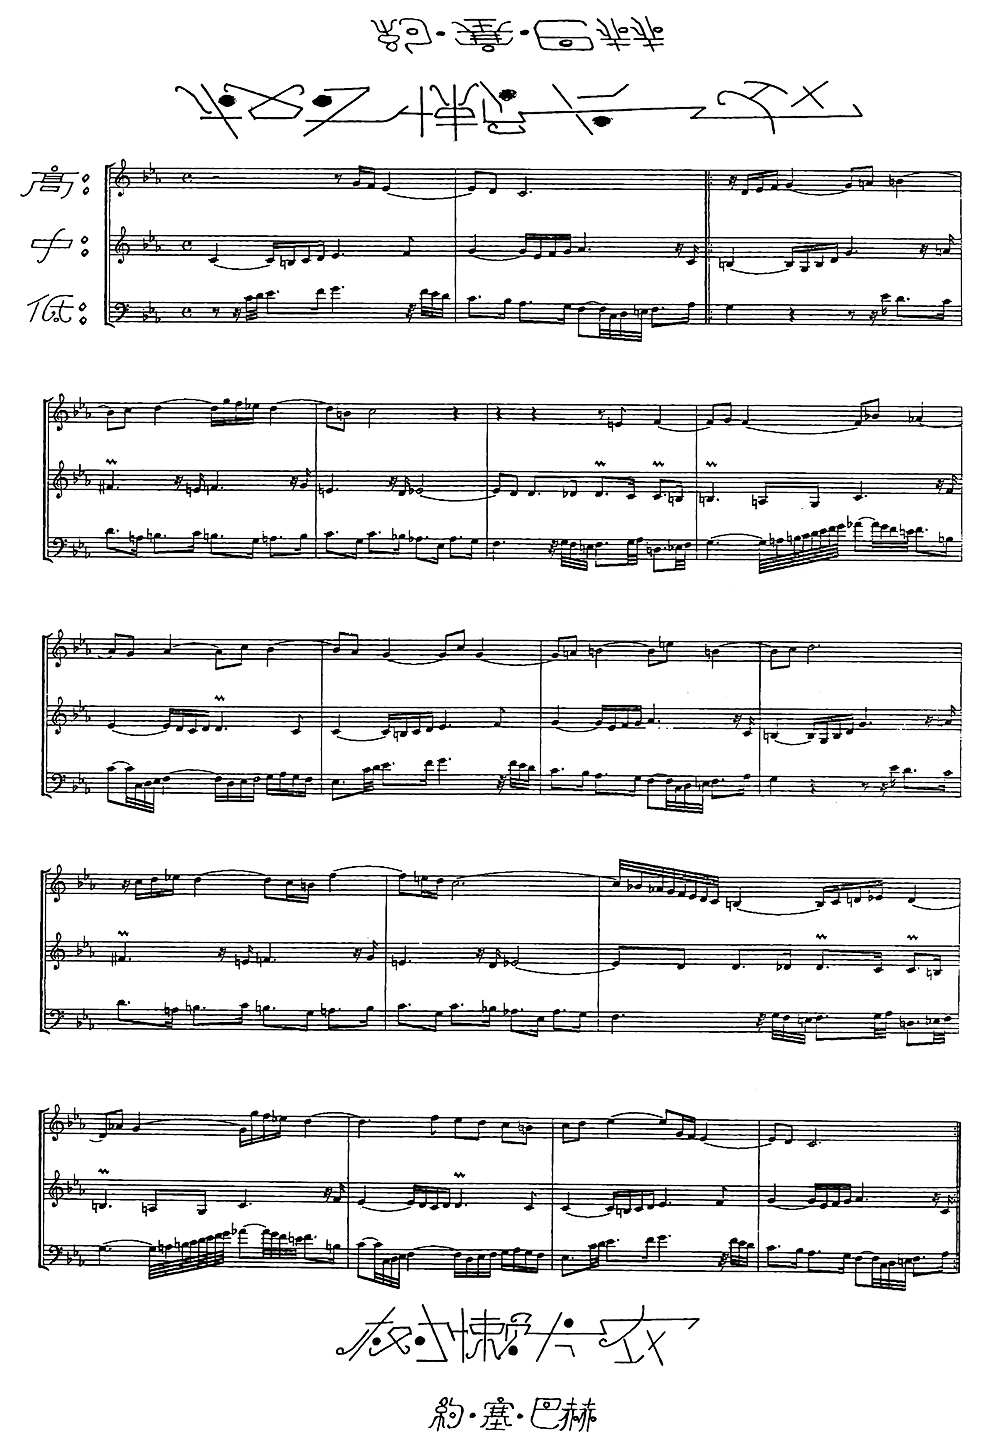
\includegraphics[height=.9\textheight]{img_133.png}
\caption[《树懒卡农》,选自巴赫《音乐的奉献》。]
  {“树懒卡农”,选自巴赫的《音乐的奉献》。[乐谱是用唐纳德·伯德的程序“斯马特”印制的,美术字由陈春光设计。]}
\end{figure}

\item[乌龟]这在他是很轻松自如的。至于“高”、“中”、“低”三个字,你一定猜得出它们指什么。

\item[阿基里斯]我想是代表“女高音”、“女中音”、“女低音”,因为三个声部的作品常常用这种方式构成。你说呢,小懒?

\item[树懒]它们不是——

\item[阿基里斯]等一下,我们三个现在呆的地方很有意思:你,小懒,位置最高,挂在树上;我在中间,坐在地上;龟兄最低,泡在下面的小塘里。哎——你怎么出来了,龟兄,还穿上了你的外套?你看去很疲倦。怎么啦?

\item[乌龟]精疲力尽了。我得先走一步。\dlnote{(步履疲惫地走远了。)}

\item[阿基里斯]他真可怜——看来他确实顶不住了。他一上午都在颠来颠去的。为了同我再较量一次,他正接受训练呢。

\item[树懒]这在他可是竭尽了全力。

\item[阿基里斯]是的,但是没用。他也许能赢一只树懒……可要想赢我——决不可能!哎,你不是要告诉我那三个字的意思吗?

\item[树懒]至于“高”、“中”、“低”三个字,你根本猜不出它们指什么。

\item[阿基里斯]要是我刚才猜得不对,这倒更让我好奇了。算啦,我们先不谈这个了。我真有点想吃东西了,我上次在老蟹那儿吃过一次油炸土豆片,听说你也会做?据说那东西有一种神奇的功效:当你觉得懒洋洋时,吃上它几片,马上就能——

\item[树懒]精力充沛了。

\item[阿基里斯]对,他们是这么说的。可是,像你这样常吃它的人,说话、办事的速度居然只是以慢吞吞而著称于世的龟兄的一半,这不免让我对这种传说产生怀疑。不过,不管怎么说,它还是挺好吃的。炸的时候有什么要领吗?

\item[树懒]你得后退一步。

\item[阿基里斯]对,这样就不会被溅出的热油烫着了,是吧?我现在就去试试,我想我会做成功的,只可惜龟兄也许尝不到了。

\end{dialogue}

\end{dialog}
